\subsection{Messung des Ankerwiderstand}

Im zweiten Versuch soll der Ankerwiderstand $R$ bestimmt werden.
Der Ankerwiderstand kann über das Ohm'sche Gesetz berechnet werden,
dafür ist eine Matrix mit den Messwerten der Spannungen und Ströme gegeben.

Da mit den Messwerten die Ströme über den Spannungen abgebildet werden ist die
Steigung nicht der Widerstand sondern der Leitwert. Deshalb muss zur Ermittlung
des Ankerwiderstand noch das Reziproke des Leitwerts berechnet werden.

\begin{equation} \label{eq121}
    \begin{split}
        R&=\frac{U_a}{I_a} \Leftrightarrow G=\frac{1}{R}=\frac{I_a}{U_a}\\
        R&\simeq 3.26 \mathrm{\Omega}
    \end{split}
\end{equation}

\begin{figure}[H]
 \centering
 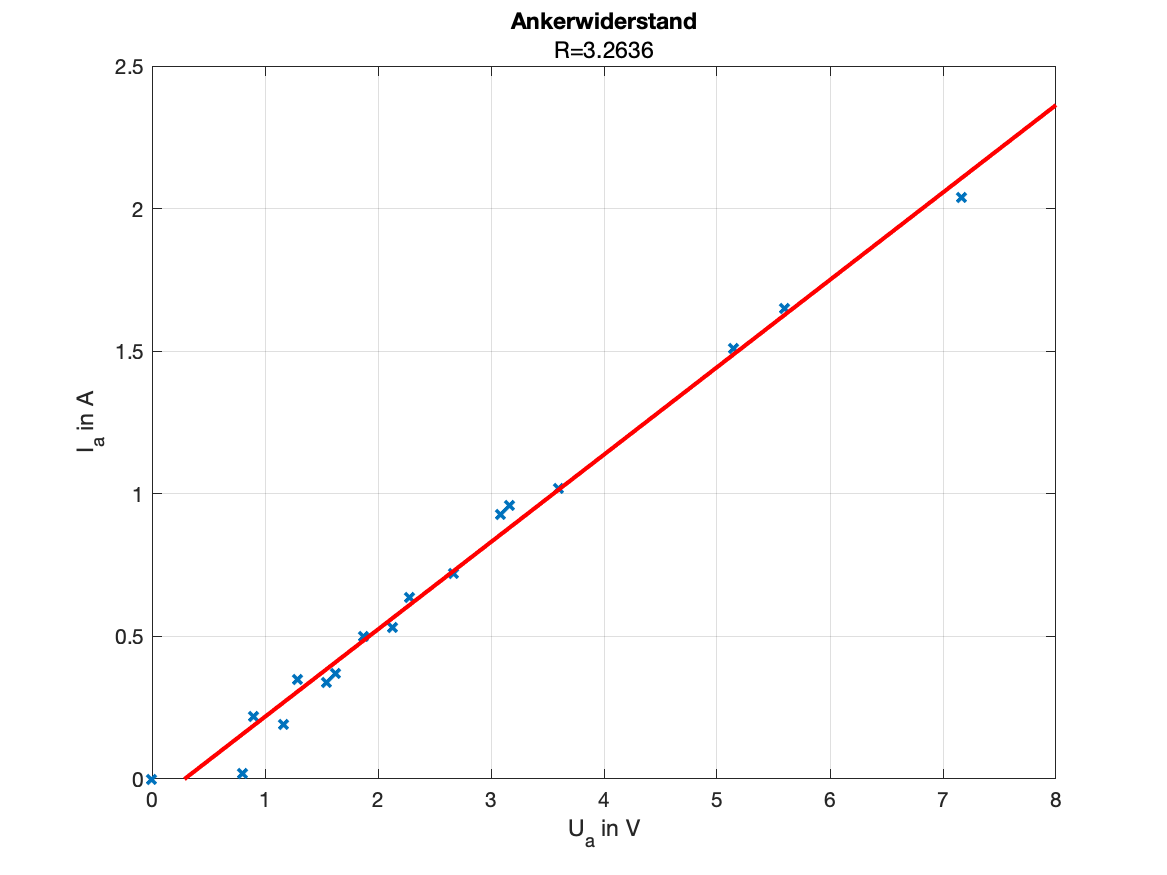
\includegraphics[width=1\textwidth]{as_labor01_2.png}
 \caption{Plot der Aufgabe 2}
 \label{fig:PlotAufgabe2}
\end{figure}